\documentclass[12pt,letterpaper]{article}
\usepackage{geometry}
\geometry{margin=1in}
\usepackage{graphicx}
\usepackage{float}

\setlength{\parindent}{0pt}
\setlength{\parskip}{0.5em}

%make lists tighter
\usepackage{enumitem}
\setlist{nolistsep}

%reduce spacing before and after section
\usepackage{titlesec}
% reduce section, subsection, etc spacing
\usepackage{titlesec}
\usepackage{amsmath, amssymb}
\titlespacing*{\section}{0pt}{0\baselineskip}{0\baselineskip}
\titlespacing*{\subsection}{0pt}{0\baselineskip}{0\baselineskip}
\titlespacing*{\subsubsection}{0pt}{0\baselineskip}{0\baselineskip}

%reduce list spacing
\usepackage{enumitem}
\setlist{nosep}

\usepackage[hidelinks]{hyperref}

\title{Lab 3.2 - FMRI, Stat 214, Spring 2025\vspace{-2em}}

% submission must not contain any of your names
% but feel free to make a version for yourself with your names on it
% \author{Your names}

\begin{document}
\maketitle


\section{Introduction}

There is a need to understand how the human brain interprets language. Functional Magnetic Resonance Imaging (fMRI) allows researchers to observe how the brain responds to language stimuli by measuring blood-oxygen level-dependent (BOLD) signals across different brain regions. This report builds on prior work by Jain and Huth (2018), who demonstrated that introducing context into word representations significantly improves the ability to model fMRI responses. 

We have explored how different word embedding strategies affect the prediction of whole-brain BOLD responses during natural story listening. In the previous lab 3.1, we evaluated the performance of three types of embeddings, Bag-of-Words, Word2Vec, and GloVe, but none could predict BOLD signals significantly effectively. 

The drawback of these methods is that they assume a one-to-one mapping between words and vectors to generate a feature matrix: in other words, they ignore the characteristic of natural language that the meaning of a word varies depending on its relationship with surrounding words. Therefore, in this lab, we attempt to generate features from text using BERT, an encoder that explicitly considers context to obtain the feature matrix. 

This report aims to verify whether the accuracy of BOLD signal prediction is improved by using more informative features from text, using BERT.

\section{Exploratory Data Analysis}

This section describes the structure and characteristics of the data used in our analysis.

There are two types of data: whole-brain blood-oxygen level-dependent (BOLD) signals measured at various points across the podcast scanned by fMRI ( treated as “response”), and the raw text for the stories (treated as “stimulus”).


The response data was collected from two anonymized subjects, “subject 2” and “subject 3,” who were scanned using fMRI while listening to the same set of 101 stories. Each fMRI scan collected the signals from 94,251 voxels for subject 2 and 95,556 voxels for subject 3, which suggests individual differences in brain structure and size. Due to this variability, it is not feasible to train a model on one subject's data and apply it directly to predict another. Hence, we decided to randomly split the data into 101 stories, using 70 stories (about 70\%) as the training data and 31 stories (about 30\%) as the test data, train the model, and make the prediction for each subject. 


The stimulus data includes the text data that has been segmented into words and the time data for when each word was played. Once word embeddings are generated from the text, these timestamps allow us to align each word with the corresponding fMRI scan time point, allowing the dimensions of the response and stimulus data to be matched.

To better understand the dataset, we performed some exploratory data analysis. For each story in the training data, the minimum and maximum word counts ranged from 697 and 3,274 respectively, while the minimum and maximum unique word counts ranged from 278 and 1,052 respectively. When the training data was totaled, there were 10,356 unique words. As discussed in the following sections, the fact of having more than 10,000 unique words leads to stimulus $X$ becoming very large and that can make ridge regression computationally expensive without appropriate dimensionality reduction strategies.


\section{Embeddings}

\subsection{BERT-Based Encoder}

In natural language processing, the encoder is an architecture that converts the input (e.g., text, audio file) into features in numerical form for quantitative analyses.

In this project, an encoder is used to extract features from 70 stories, and the training data for modeling ridge regression predicts the BOLD signal (modeling of ridge regression is discussed in the next section).

We want to obtain informative features from the stories for a better prediction. However, Bag-of-Words, Word2Vec, and GloVe, which were used in the Lab 3.1 analysis, just convert each word in a sentence into a vector, so they cannot reflect the contextual meaning of each word in the features. For example, the word "model" has a different meaning in the sentence "Train a machine learning model" than in the sentence "He is a fashion model," but the model that converts a word directly into a vector cannot express the difference in meaning with features.

To deal with this problem, we will train a BERT (Bidirectional Encoder Representations from Transformers) model to obtain informative features, including the words' contextual meaning. BERT gives contextual meaning to words through a mechanism called "attention." Attention uses three matrices, query, key, and value, to add meaning to the vector generated from each token based on its relationship to other words that are strongly related to that.

Let us discuss this mathematically. Let $X$ be the input matrix (set of the vectors generated from each token) and $Q, K, V$ be the query, key, and value matrices. The dimension is $X \in \mathbb{R}^{n \times d}$ and  $Q, K, V \in \mathbb{R}^{d \times d}$, where $n$ is the number of the tokens in the text and $d$ is the dimension of the embedding. Since the BERT tokenizer has 30,522 different tokens (i.e., the original vector assigned for each token is $\mathbb{R}^{30522}$), $X$ becomes $\mathbb{R}^{n \times d}$ by getting the matrix product of $\mathbb{R}^{30522 \times d}$ to each token. (Similarly, to compute the predicted probability, a linear mapping of $\mathbb{R}^{d \times 30522}$ is performed on the $\mathbb{R}^{d}$ vector that is the feature of each token.)

\begin{align*}
\tilde{Q} &= XQ \in \mathbb{R}^{n \times d}\\
\tilde{K} &= XK \in \mathbb{R}^{n \times d}\\
\tilde{V} &= XV \in \mathbb{R}^{n \times d}\\
A &= \text{softmax}\left(\frac{\tilde{Q}\tilde{K}^T}{\sqrt{d}}\right) \in \mathbb{R}^{n \times n}\\
O &= A\tilde{V} \in \mathbb{R}^{n \times d}
\end{align*}

Here, $A$ reflects the relationship between two tokens by getting an inner product of the two vectors. Transformer aggregates the information of each token contained in $\tilde{V}$ with the weight computed by $A$ and adds the information to the original vector by residual connection, which allows each token to have its contextual meaning. In addition, multi-head attentions have multiple $Q, K, V$s to capture the relationship between words from various perspectives.

One attention block is constructed by the attention structure and feed-forward by fully connected layers. BERT consists of multiple attention blocks in a concatenated form to reflect complex contextual relationships in the feature.

In our analysis, we converted sentences into a set of tokens using the trained tokenizer “bert-base-uncased.” We then trained a BERT model to obtain a feature matrix from the tokens (see the next section for details on the training process and hyperparameter tuning).

For the input strings, it is necessary to define batches of appropriately cut chunks of text for each story. However, if we cut the story only based on the length of the words, most batches are cut off at times regardless of meaning and grammar, so they are not understandable as sentences on their own anymore. Therefore, we decided to utilize the time data for each word played. We defined "sentence breakpoints" where the time difference between the words played before and after was long and cut the sentence there. Specifically, the following rules were established: (i) more than 0.7 seconds have passed since the previous word was uttered, (ii) the previous sentence has at least 30 words (if it is less than that, it is not cut), and (iii) when the sentence exceeds 100 words, it is automatically cut (very rare case). We found that many batches become sentences that make sense as stand-alone by taking this approach.

To align the dimension of the feature matrix with the number of fMRI scans, we averaged the feature vectors of tokens corresponding to each word, then downsampled using the data of when words were spoken and fMRI scans were performed. The former operation averaged features only when two or more tokens corresponded to a single word. The latter operation is identical to the downsampling process in lab3.1. Finally, we created a matrix with lags [1,2,3,4] for each row of the embedding and to get the covariates which explicitly consider that subjects retain information for a long time.

\subsection{Masked-Language Model Training}

For training our BERT-based encoder, we implemented a masked language modeling (MLM) approach, which is the primary pre-training objective of the original BERT model. The MLM task involves randomly masking some tokens in the input sequence and then training the model to predict these masked tokens based on the surrounding context. So, instead of predicting the following word, we mask a word in the middle and ask the model to guess the word given the words on both sides. This method thus allows the model to see both the right and left context. This is crucial for capturing the full contextual meaning of words that the previous embedding methods used in Lab 3.1 could not achieve.

The masking process follows a specific strategy:

\begin{itemize}
    \item 15\% of tokens are selected for potential masking
    \item Of these tokens:
    \begin{itemize}
        \item 80\% are replaced with the special [MASK] token
        \item 10\% are replaced with a random token from the vocabulary
        \item 10\% remain unchanged
    \end{itemize}
\end{itemize}

More specifically, each masked token is handled according to the 80-10-10 strategy.

\begin{itemize}
         \item 80\% of the selected tokens are replaced with the special [MASK] token Example: "well i'm in uh bergen belsen concentration camp" → "well i'm in uh [MASK] belsen concentration camp"
    
        \item 10\% of the selected tokens are replaced with a random token from the vocabulary Example: "well i'm in uh bergen belsen concentration camp" → "well i'm in uh years belsen concentration camp"
        \item  10\% of the selected tokens remain unchanged Example: "well i'm in uh bergen belsen concentration camp" → "well i'm in uh bergen belsen concentration camp"

   
\end{itemize}



This masking approach is important for two main reasons: First, it prevents the model from learning to only predict when it sees a [MASK] token (since in real usage, there won't be mask tokens). Second, by occasionally replacing words with random ones, the model learns to be more robust to noise and errors in the input. This approach helps the model develop more generalized contextual representations that better capture the semantics of language as it appears in the fMRI stories.



Our implementation of the masking process is as follows:
\begin{enumerate}
    \item Selecting tokens for masking using a probability matrix where each token has a 15\% chance of being selected.
    \item Ensuring padding tokens are excluded from masking by setting their probability to zero.
    \item For the selected tokens, determining their treatment based on the 80/10/10 rule.
    \item Maintaining a separate labels tensor that contains the original token IDs only at masked positions (all other positions are set to -100, which is ignored in the loss calculation).
\end{enumerate}


We trained our encoder on the actual story data from the fMRI dataset, rather than using external text corpora (just mentioned in `train\_encoder.py` as a example). This ensures that our embeddings capture the specific patterns present in the stories used in the fMRI experiments, which should lead to better performance in ridge regression task.

\subsection{Hyperparameter Tuning}

\subsubsection{Data for hyperparameter tuning}

This project consists of two models: an encoder model and a ridge regression model, each requiring hyperparameter tuning. We divided the entire dataset into 70\% training data and 30\% test data, then used 30\% of the training data ($\simeq$ about 20\% of the total data) as evaluation data for parameter tuning. After that, we retrained the encoder using all of the training data and then re-divided the training data into model training and evaluation for tuning ridge regularization parameters.

As a result, a partition of the evaluation data for the ridge hyperparameter tuning was also used to train the encoder. This was done after considering the benefits of training the encoder with a large amount of data, given the limited amount of text data, and the benefits of finding optimal parameters with a realistic amount of computation.

If we have independent evaluation data for both the encoder and ridge regression, the amount of data available for training the encoder becomes small. On the other hand, if we interpret the encoder and ridge regression as a single system and attempt to tune all hyperparameters at once, not only does the computational complexity for training and evaluating a single set of hyperparameters increase but also the number of candidate parameter sets increases exponentially. 

Mathematically, when the number of elements in the encoder's parameter set is $x$ and those in the ridge parameter set are $y$, the total parameter set becomes $xy$, meaning that the ridge model must be trained at least $xy$ times. This increase in computational complexity needs to be mitigated by tuning fewer parameters.

As a result, we decided to divide the training data into training and evaluation data each time and perform thorough parameter tuning. This enabled us to achieve optimal encoder parameters while maintaining sufficient data for ridge regression tuning. Note that the data used for the test is not used for training or evaluation, so there is no data leakage for testing.

\subsubsection{Hyperparameters of the encoder}
We conducted hyperparameter tuning to optimize our BERT-based encoder for the fMRI prediction task. The key hyperparameters and the original settings are:

\begin{enumerate}
    \item \textbf{Model Architecture Parameters}
    \begin{itemize}
        \item Hidden size: 256 
        \item Number of attention heads: 4 
        \item Number of layers: 4 
        \item Intermediate size in feed-forward networks: 512 
    \end{itemize}
    
    \item \textbf{Training Parameters}
    \begin{itemize}
        \item Batch size: 8
        \item Learning rate: 5e-4
        \item Maximum sequence length: 32
        \item Number of epochs: 3
        \item Masking probability: 15\%
    \end{itemize}
\end{enumerate}

Considering the limited amount of the text data for training the model, we chose a smaller model architecture than the original BERT-base. The smaller architecture still captures contextual relationships while being more efficient to train and use for subsequent ridge regression modeling.

For optimization, we used the AdamW optimizer, which combines the Adam optimization algorithm with weight decay regularization. We trained the model on CPU due to resource constraints, with a 70-30 train-validation split of our story data. 

When we trained the model with the original parameter setting, it required significant computational resources. The full training process took approximately 29 minutes on CPU, with each epoch requiring about 9 minutes to complete, resulting in following training/validation loss curves.


\begin{figure}[H]
  \centering
  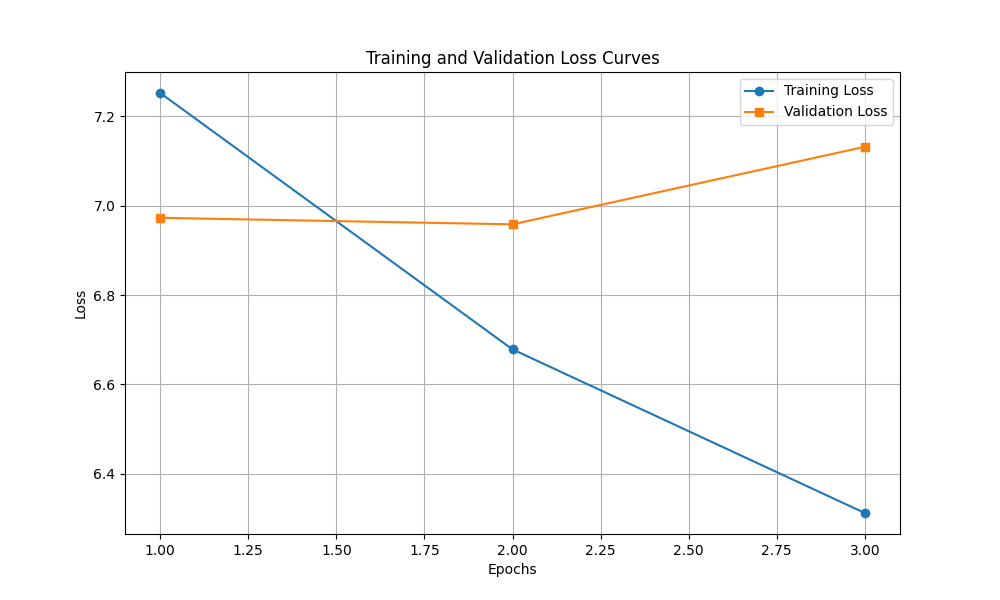
\includegraphics[width=1\textwidth]{bert_loss_curves.png}
  \caption{Training and validation loss curves for the BERT-based encoder across three epochs}
  \label{fig:mlm_loss}
\end{figure}

 In Figure 1, we noticed that the training loss decreases as epoch increases, whereas the validation loss increases in the third epoch. It suggests that we also need to consider the best number of epoch, as the model easily suffers from overfitting.


We will discuss the use of hyperparameter searching and the loss curves in the next section.


\subsubsection{Hyperparameter tuning}

The full range of hyper-parameters under consideration are hidden size, number of heads, number of layers, intermediate size, maximum length, number of epochs, learning rate and mask probability. Note that in our analysis, we only consider one mask probability (mlm\_prob = 0.15). Additionally, we set an upper bound of 10 epochs, and then visually determine the optimal number of epochs based on evaluation loss. 

Based on the original BERT paper and Google's best practices for hyperparameter tuning shown in the references section, we identified several reasonable hyperparameter ranges that would be possible under time and computational constraints. These are shown below in Table 1.

\begin{table}[H]
    \centering
    \renewcommand{\arraystretch}{1.25}{\fontsize{11}{12}\selectfont
    \begin{tabular}{|p{3.5cm}|p{2cm}|p{3cm}|p{6cm}|}
        \hline
          & \textbf{Chosen Range} & \textbf{Typical Range} & \textbf{Notes} \\
        \hline
        \textbf{Hidden Size} & \{128, 256, 512\} & \{128, 256, 512, 768\} & BERT-base uses 768. Smaller sizes reduce model complexity and training time.  \\
        \textbf{Number of Heads} & \{4\} & \{4,8,12\} & Hidden size must be divisible by number of heads. BERT-base uses 12 heads but we choose 4 to reduce model complexity and training time.  \\
        \textbf{Number of Layers} & \{2,...,6\} & \{2,...,12\} & BERT-base uses 12 layers. Smaller number of layers may be more effective for smaller datasets such as ours so we choose a 2-6 range.  \\
        \textbf{Intermediate Size} & 4 * Hidden Size & 4 * Hidden Size & Common practice is to choose intermediate size = 4 * hidden size.  \\
        \textbf{Learning Rate} & [$1e-5$, $5e-5$] & [$1e-5$, $5e-5$] & Lower learning rates such as $2e-5$ or $3e-5$ are commonly effective for fine-tuning BERT models.  \\
        \hline
    \end{tabular}
    \caption{Chosen and Typical Hyperparameter Ranges}
    }
    \label{tab:accuracy_values}
\end{table}


For hyperparameter tuning implementation, the first thing to note is that we split the training data into a training set and evaluation set. For every hyper-parameter candidate set, we fit the encoder model based on the selected hyper-parameters (using the Python package Optuna), and plot the training and evaluation loss. We then select the hyperparameter set that minimizes the evaluation loss in order minimize overfitting while maximizing encoder model performance. Next, we observe each plot to identify the number of epochs that minimizes evaluation loss. 

Our top and worst candidate hyperparameter sets are shown below along with their training/evaluation loss curves.

%\begin{table}[H]
%    \centering
%    \renewcommand{\arraystretch}{1.25}{\fontsize{11}{12}\selectfont
%    \begin{tabular}{|p{4cm}|p{8cm}|p{2cm}|p{2cm}|}
%        \hline
%          & \textbf{Hyperparameters} & \textbf{Evaluation Loss} & \textbf{Loss Curves} \\
%        \hline
%        \textbf{Hyperparameter Set 1} & \{Hidden Size= 512, Number of Heads = 4, Number of Layers = 4, Learning Rate = 1.3458811443604462e-05, Number of Epochs = 2\} & 6.8925 & Figure 2 \\
        %\textbf{Hyperparameter Set 2} & \{Hidden Size = 512, Number of Heads = 4, Number of Layers = 4, Learning Rate = 1.3458811443604462e-05, Number of Epochs = 1\} & 6.8945 & Figure 2\\
        %\textbf{Hyperparameter Set 3} & \{Hidden Size = 512, Number of Heads = 4, Number of Layers = 2, Dropout = 0.1670905276622703, Learning Rate = 2.4304583449362825e-05, Number of Epochs = 2\} & 6.9337 & Figure 3 \\
        %\textbf{Hyperparameter Set 4} & {Hidden Size = 512, Number of Heads = 4, Number of Layers = 2, Learning Rate = 2.4304583449362825e-05, Number of Epochs = 1} & 6.9366 & Figure 3\\
        %\textbf{Hyperparameter Set 5} & {Hidden Size = 512, Number of Heads = 4, Number of Layers = 4, Learning Rate = 1.3458811443604462e-05, Number of Epochs = 3} & 6.9939 & Figure 2 \\
        %\textbf{...} & ... & ... & ... \\
        %\textbf{Hyperparameter Set n} & {Hidden Size = 256, Number of Heads = 4, Number of Layers 5, Learning Rate = 3.0971755250404505e-05, Number of Epochs = 8} & 9.6497 & Figure 4
% \\
%        \hline
%    \end{tabular}  
%    \caption{Hyperparameters per hyperparameter set}
%    }
%    \label{tab:accuracy_values}
%\end{table}


\begin{table}[H]
\centering
\begin{tabular}{|l|c|c|c|c|c|c|c|}
\hline
\textbf{Rank} & \textbf{Hidden} & \textbf{Heads} & \textbf{Layers} & \textbf{Learning rate} & \textbf{Epochs} & \textbf{Eval.\ loss} \\
\hline
Top 1 & 512 & 4 & 4      & 1.3459e-05 & 2 & 6.8925 \\
\hline
Top 2 & 512 & 4 & 2  & 2.4305e-05 & 2 & 6.9337 \\
\hline
Worst  & 256 & 4 & 5      & 3.0972e-05         & 8 & 9.6497\\
\hline
\end{tabular}
\caption{Hyperparameter settings and evaluation loss for the top two models.}
\label{tab:hyperparams}
\end{table}



%From Figure 2, we observe the training and evaluation loss curves. We can see that the training loss decreases as we increase the number of epochs. Additionally, we observe that the evaluation loss decreases to a minimum and begins increasing as we add more epochs. By selecting the epoch level at evaluation loss minima (epoch=2), we tune the epoch-level. This follows similarly for Figure 3 and Figure 4.

The following plot, Figure 2 shows the progression of the training and validation loss over the various epochs of our best set of hyperparameters. It can be seen that the ideal state can be reached after just two epochs, after which a rapid overfitting occurs.
    
\begin{figure}[H]
    \centering
    \includegraphics[width=0.8\linewidth]{best_best_hyperparameters.jpg}
    \caption{Training and Evaluation Loss of the best model}
    \label{fig:enter-label}
\end{figure}

\section{Modelling and Evaluation}

This section assumes that the report on Lab 3.1 has already been studied, where an embedding was created using the methods Word2Vec, GloVe and bag-of-words. On the basis of these embeddings, a ridge model was trained, which uses the embeddings to predict the reactions of the brain using blood-oxygen level-dependent signals across different brain regions (voxels). We follow the same goal in the modeling part, but we use the resulting embedding based on the previous sections. The basic methodology used here is equivalent to Lab 3.1, so that the results of the different embeddings remain comparable.

\subsection{Modelling}
For modeling, we again use the ridge model that predicts the different blood-oxygen levels at the voxel level. The ridge model is optimized using a hyperparameter search, which selects the best parameters for the ridge model at voxel level. 

The ridge model achieves the following results with BERT-based embedding:


\begin{figure}[H]
  \centering
  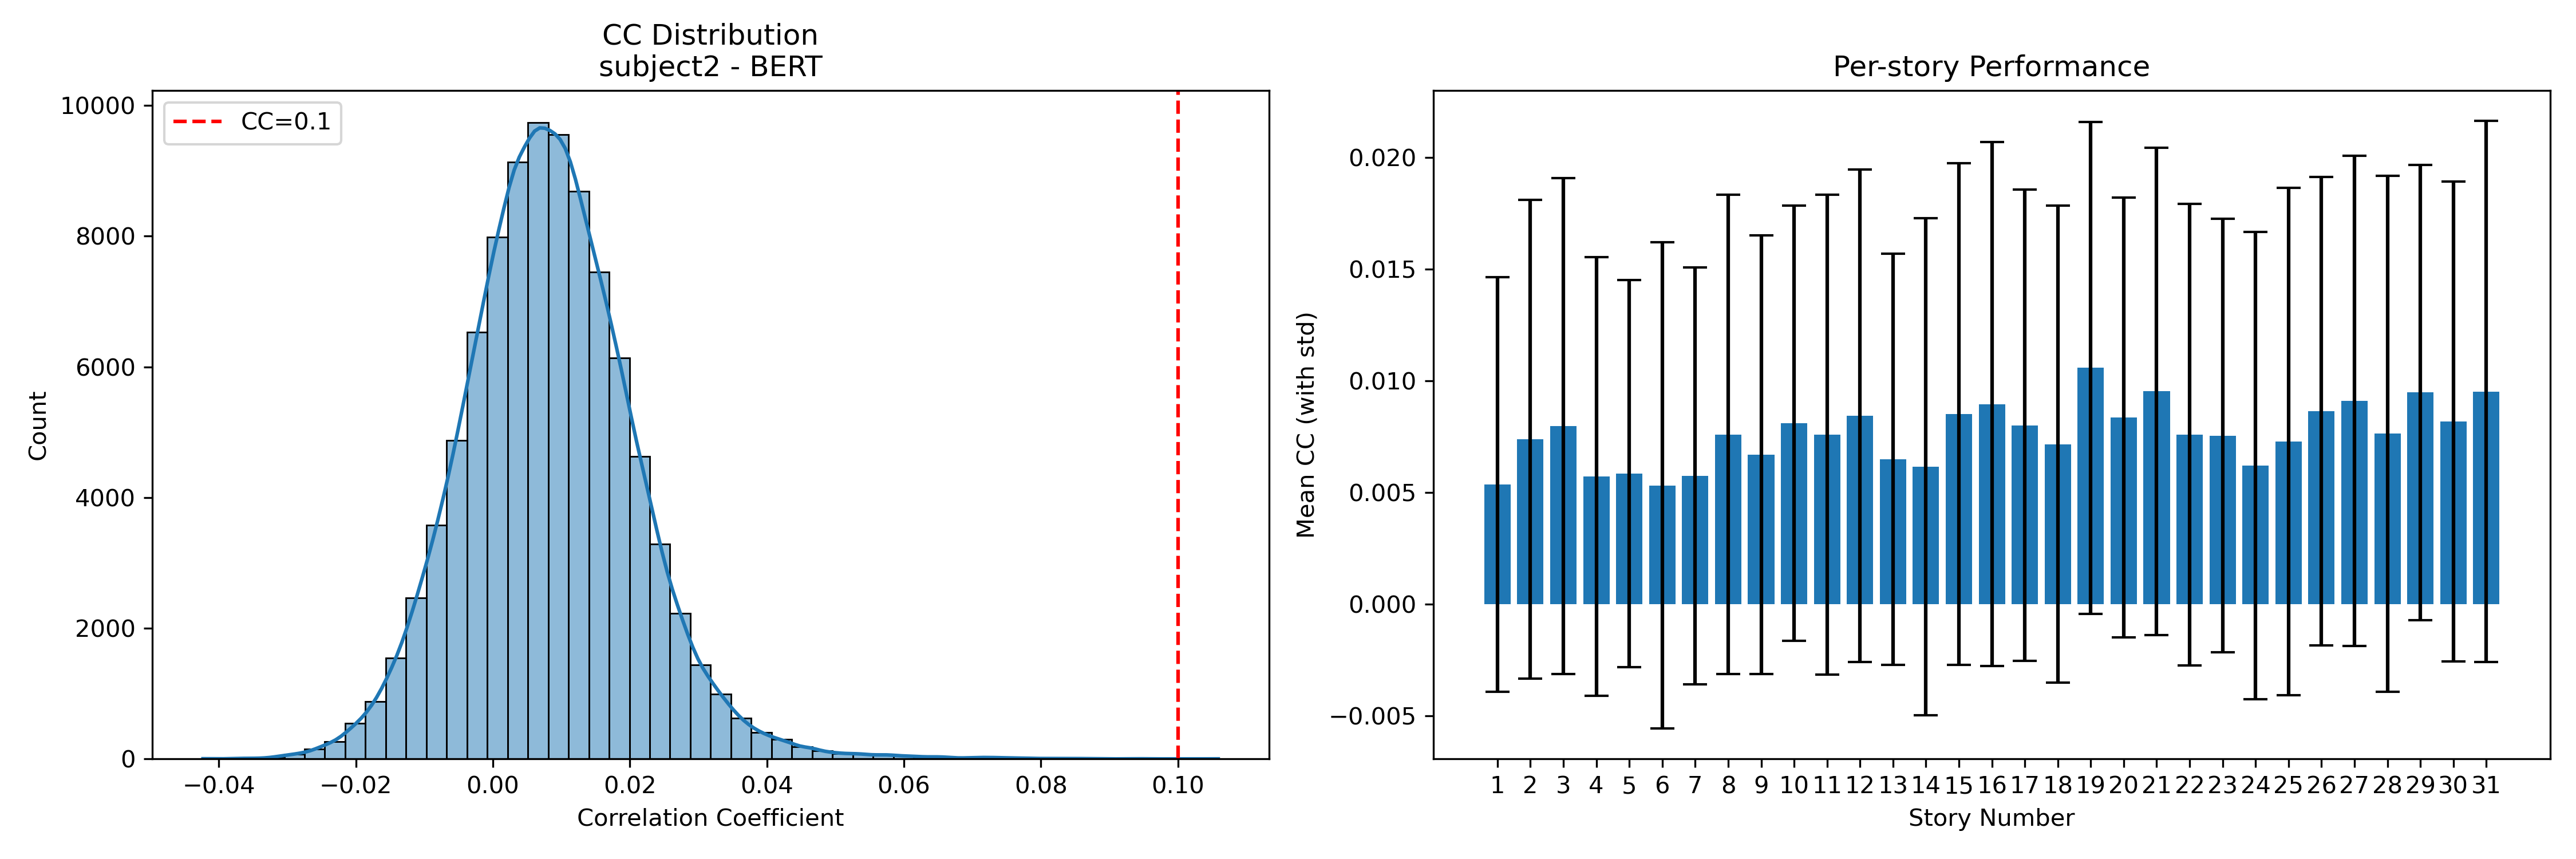
\includegraphics[width=0.8\textwidth]{subject2_BERT.png}
  \caption{Evaluation of the Ridge Model with BERT embedding on Subject 2}
  \label{fig:evaluation_ridge_bert_subject2}
\end{figure}

\begin{figure}[H]
  \centering
  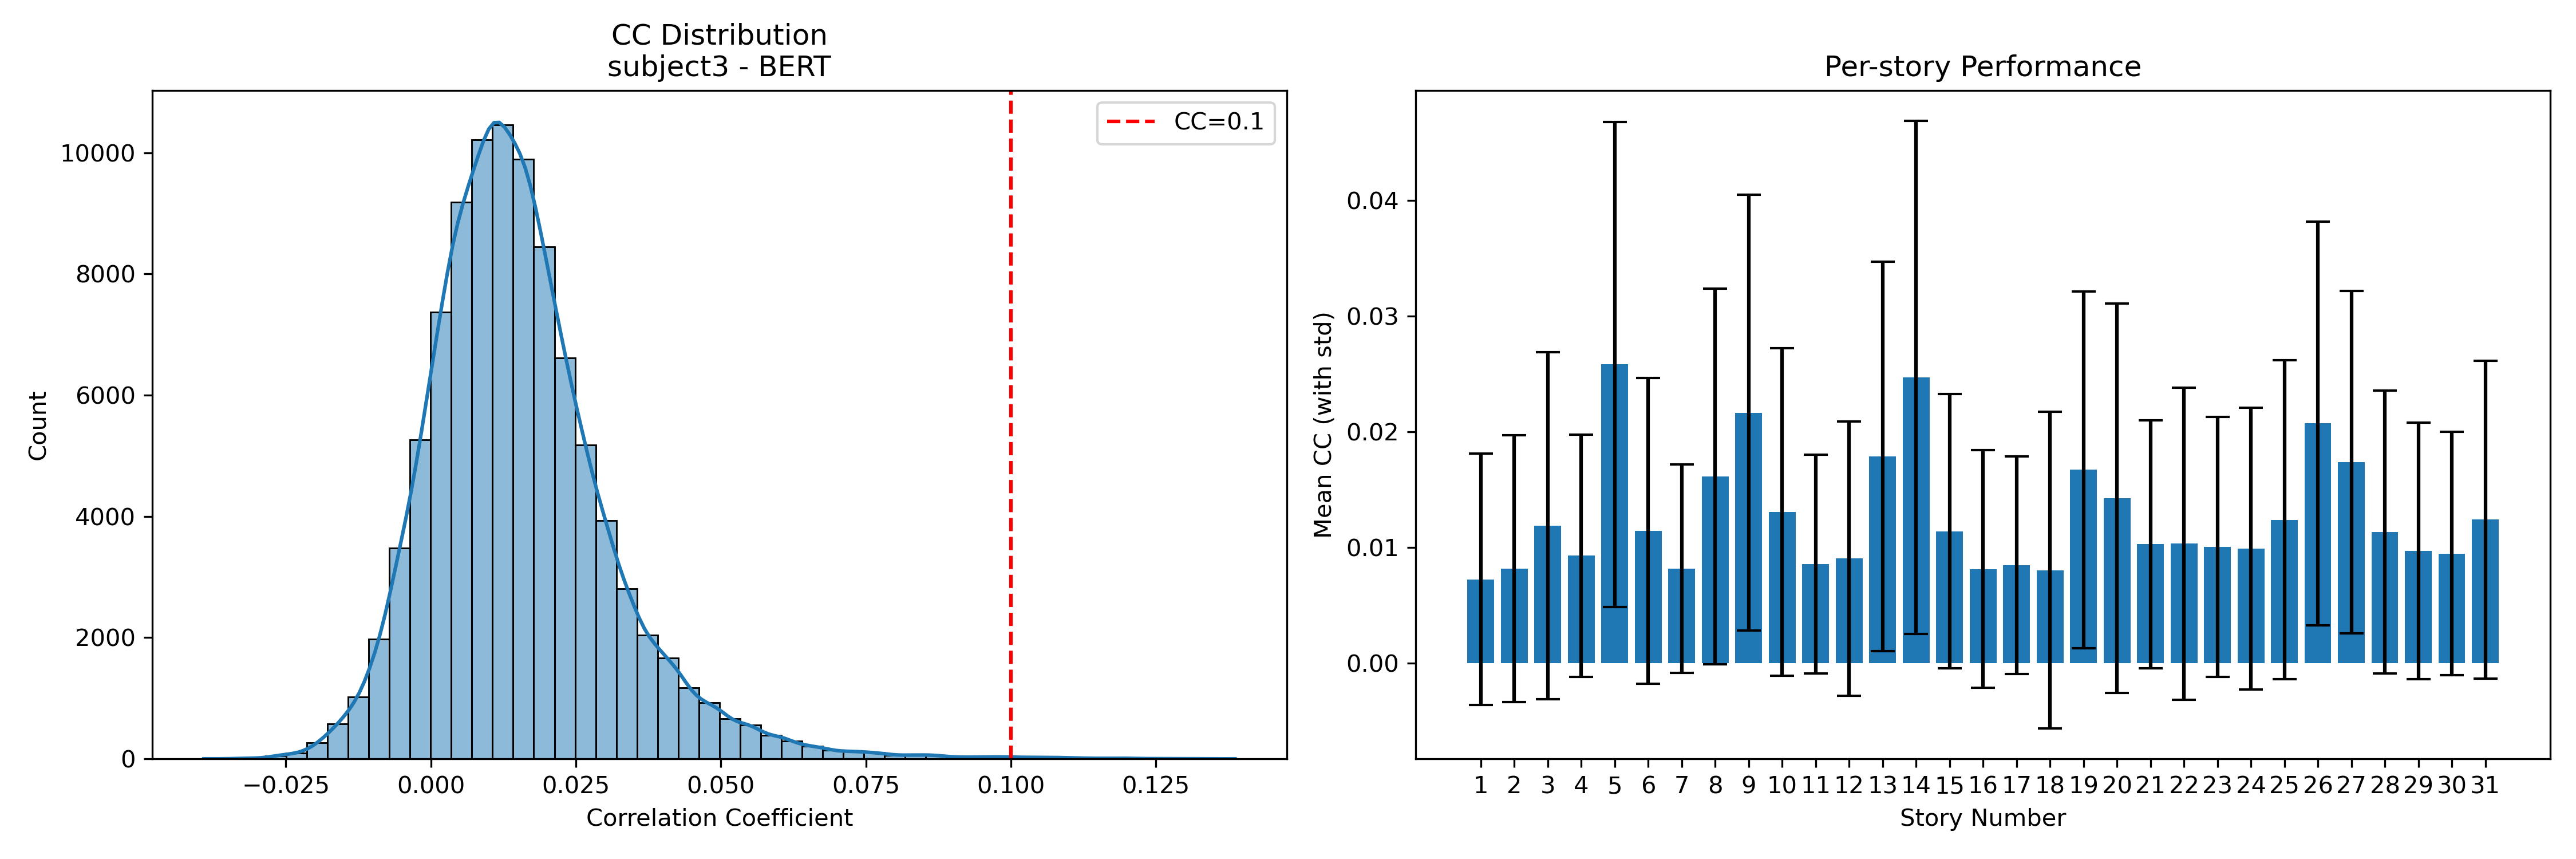
\includegraphics[width=0.8\textwidth]{subject3_BERT.png}
  \caption{Evaluation of the Ridge Model with BERT embedding on Subject 3}
  \label{fig:evaluation_ridge_bert_subject3}
\end{figure}

The above plots clearly shows that the results are pretty similar to the results of the embeddings from Lab 3.1, but still a very weak correlation without a value over 0.1 according to the PCS schema. Overall, we can only recognize a weak correlation for 0.05\% of the voxels over both subjects and it perform pretty bad over all voxels.

\subsection{Comparison with other Embeddings}

In the following Table~\ref{tab:accuracy_values}, we can see the comparison of all embeddings with respective Mean Correlation-Coeffitient (CC), the Top 5\% CC and the Top 1\% CC:

\begin{table}[H]
    \centering
    \begin{tabular}{l c c c c}
        \hline
          & \textbf{bag-of-words} & \textbf{Word2Vec} & \textbf{GloVe}  & \textbf{BERT} \\
        \hline
        \textbf{Mean CC Subject 2} & 0.0091 & 0.0101 & 0.0097 & 0.0092 \\
        \textbf{Mean CC Subject 3} & 0.0138 & 0.0162 & 0.0147 & 0.0163 \\
        \textbf{Top 5\% CC Subject 2} & 0.0355 & 0.0356 & 0.0317 & 0.0293 \\
        \textbf{Top 5\% CC Subject 3} & 0.0490 & 0.0498 & 0.0431 & 0.0460 \\
        \textbf{Top 1\% CC Subject 2} & 0.0565 & 0.0525 & 0.0457 & 0.0426 \\
        \textbf{Top 1\% CC Subject 3} & 0.0782 & 0.0747 & 0.0640 & 0.0669 \\
        \hline
    \end{tabular}
    \caption{Correlations Coefficient per subject for different embedding models}
    \label{tab:accuracy_values}
\end{table}

From above, it can seen that they are all relatively in the same range and that we were not able to achieve a significantly better performance with our BERT model. Also the model show similar bad results over all voxels than our previous embeddings. This is surprising, as a better embedding is to be expected with a modern approach, which subsequently enables us to make better predictions.

\section{Conclusion}
In this report, we have implemented a modern BERT model for embedding stories and subsequently used this embedding for the prediction of fMRI BOLD signals. This extends our previous work in Lab 3.1. The hyperparameter search for embedding showed that it only takes few epochs before the validation loss increases again. This indicates that an ideal state is quickly reached in the BERT model due to the small amount of data. 

When using the BERT embeddings with ridge regression to predict BOLD signals across voxels, we found no performance improvement compared to the simpler Word2Vec, GloVe, and bag-of-words embeddings from Lab 3.1. In fact, BERT embeddings (mean CC of 0.0092 for Subject 2 and 0.0163 for Subject 3) performed slightly worse than Word2Vec, GloVe and bag-of-word. This pattern held consistently across both the mean correlation values and the top percentile analyses. This negative result is significant, suggesting that the limitations in prediction accuracy may not stem from the embedding quality alone. So, even with the modern approach of the BERT model, it is still not possible to speak of a correlation between the measured values and the prediction of the ridge model.

Overall, this is probably due to the small size of our data set, which makes the training of BERT difficult along with many parameters of the model, as well as the small number of training cases and the limited possibilities of a ridge model in prediction.

\section{Bibliography}

Jain, Shailee, and Alexander Huth. “Incorporating Context into Language Encoding Models for FMRI.” 

\section{Collaborators} 

I certify that I have only collaborated with my group members. 


\section{Academic honesty}
To: Bin Yu 

I declare that the work presented in Lab 3.1 is entirely my own and my group members. We ourself designed and performed all the data analysis, methods and procedures presented in this report. We ourself wrote all the texts, wrote codes embeddings, modeling, and produced all the figures in this report. We used codes provided by GSI. We have included and documented all the procedures in the workflow and the results are fully reproducible. Wherever we included the work from others, we cited the sources and in 'References section', especially for equations. We used LLM specifically for improved grammar for report writing style.

By submitting this lab report and all github material, I certify that we have complied with the academic integrity standards as set in lab 3.1 instructions. 

\section{References}

\begin{itemize}
    \item \href{https://web.stanford.edu/~jurafsky/slp3/11.pdf}{https://web.stanford.edu/~jurafsky/slp3/11.pdf}
    \item \href{https://www.youtube.com/watch?v=kCc8FmEb1nY&t=1223s}{https://www.youtube.com/watch?v=kCc8FmEb1nY&t=1223s}
     \item \href{https://huggingface.co/docs/transformers/en/tasks/masked_language_modeling}{https://huggingface.co/docs/transformers/en/tasks/masked_language_modeling}
     \item \href{https://datascience.stackexchange.com/questions/64583/what-are-the-good-parameter-ranges-for-bert-hyperparameters-while-finetuning-it}{https://datascience.stackexchange.com/questions/64583/what-are-the-good-parameter-ranges-for-bert-hyperparameters-while-finetuning-it}

     \item \href{https://arxiv.org/abs/1810.04805}{https://arxiv.org/abs/1810.04805}

     \item \href{https://arxiv.org/abs/1905.05583}{https://arxiv.org/abs/1905.05583}


    
    
\end{itemize}


\end{document}
